\documentclass[a4paper,11pt, oneside]{book}
\usepackage[utf8]{inputenc}
\usepackage[francais]{babel}
\usepackage[T1]{fontenc}
\usepackage{graphicx}
\usepackage{float}
\usepackage{wrapfig}
\usepackage{setspace}
\usepackage{geometry}
\usepackage{hyperref}
\usepackage{multicol}
\usepackage{etoolbox}
\usepackage{color}
\usepackage[explicit,pagestyles]{titlesec}
\usepackage[absolute,overlay]{textpos}
\usepackage{fancyhdr}
\usepackage{fontspec}
\usepackage{eurosym}
\usepackage{titlesec}


% ====== CONFIG ========

\setmainfont{Roboto Light}

\setmainfont{Roboto Light}
\setsansfont{Roboto}
\setmonofont{Roboto}
\newfontfamily\light{Roboto Slab Light}
\graphicspath{{img/}}
\setlength{\unitlength}{1mm}

\makeatletter

\definecolor{primary}{RGB}{44, 62, 80}


\titleformat{\chapter}[display]{\huge}{\thechapter \quad #1}{0pt}{}
\titlespacing{\chapter}{0pt}{0pt}{0pt}

\titleformat{\section}[display]{\LARGE}{}{0pt}{\thesection \quad #1}


\setlength{\TPHorizModule}{1mm}
\setlength{\TPVertModule}{1mm}
\def\sizeMedia{38}
\def\size{3.8cm}
\def\sizeMargin{0.2cm}
\def\margin{2}
\def\fixMargin{0}

\pagestyle{plain}


\title{Compte rendu d'activité}
\author{Yann Prono}
\date{\today}

\def\school{TELECOM Nancy}
\def\schoolAddress{193 Avenue Paul Muller}
\def\schoolPostalCode{54602}
\def\schoolCity{Villers-lès-Nancy}
\def\schoolCodeAndCity{\schoolPostalCode, \schoolCity}
\def\schoolYear{2016 - 2017}

\def\appName{The Octopus Challenge}
\def\octopusName{Lord Octopus}

\def\club{Club Studio}
\def\chair{Eliot GODARD}
\def\secretary{Yann PRONO}
\def\banker{Ansel GAMET}
\def\teacher{Isabelle HEUDIARD}
\def\bde{Victor CHOLLEY-BARROYER}

\def\schoolYear{2016 - 2017}

% ====== END CONFIG ========


\begin{document}

	\begin{titlepage}
		\thispagestyle{empty}

{\color{primary}



\includegraphics[width=4.0cm]{img/school-logo.eps}
\hspace{9mm}

\includegraphics[width=4.0cm]{img/collegium-logo.eps}
\hspace{5mm}

\includegraphics[width=4.0cm]{img/university-logo.eps}

\vspace{0.5cm}

	\begin{center}


			{\color[rgb]{0.8,0.8,.8}\rule{\textwidth}{0.8pt}}
			\vspace{0.5cm}

			\baselineskip=3pt
			{\Huge \bfseries{\appName}}\\
			\vspace{0.2cm}
			{\huge \bfseries{English project}}
			\vspace{0.5cm}

		{\color[rgb]{0.8,0.8,.8}\rule{\textwidth}{0.8pt}}
		\vspace{0.5cm}


		
\includegraphics[width=0.6\textwidth]{logo.png}

		\Large{Yannick Philippe}\\
		\Large{Yann Prono}

		\vspace{1.5cm}
		\large{\schoolYear}
	\end{center}

}

	\end{titlepage}


	\newpage

	\newpage\null\thispagestyle{empty}\newpage
	\setcounter{page}{1}
	\tableofcontents

	\chapter{Introduction}

Is this the fiftheen time you passed the TOEIC test and you still didn't get it ?
Are you bored about making uninteresting tests on abandoned websites?
Do you want to improve your english level by listening dialogs of your preferred TV serie ?
Do you want to challenge others people about your language skills ?
Do you sing songs that you don't understand ?\\

\noindent English is everywhere: music, TV series, movies, articles, documentation, comics strip, social networks, youtube videos etc...
All these supports are gold nuggets. Indeed, a lot of people use these media in their daily lives in their native language.
Due to success of all these media and the utility for people, it can be possible to use some of them in order to learn a new language.\\

\noindent \appName \ is a quiz developped in the english courses context. It has been developped by students for students who wants to test a new way to learn english.
Rules are simple: you have to answer a set of questions about general culture, grammar, listening comprehension, vocabulary... If you answer wrong 3 times, you lose and have to play again since the beginning of the quiz.
At the end of a quiz session, you have the possibility to share your score with others and measure your evolution.
In order to not be bored about the application, users have to possibility to suggest questions to expand the quiz.

\setcounter{page}{1}
	\clearpage


\chapter{User documentation}
	\appName \ is a quiz application about the English culture.\\
	Now we will present you how to use the application. The application is available at the following url:
	\href{https://octopus-challenge.herokuapp.com/}{https://octopus-challenge.herokuapp.com/}
	for the next of the presentation of the application, we use this plan:
	\begin{itemize}
		\item Navigation menu
		\item Home page
		\item How to play the game
		\item Best scores
		\item Send a question request\\
	\end{itemize}

	\section{Navigation bar}
	The navigation menu was placed on the top of each page of the web site and this offer for the player five Buttons to navigate into the different screens(Figure 1).


	\begin{center}
		\begin{figure}
			\centering
			
\includegraphics[width=1\textwidth]{CNave.png}
			\caption{The navigation bar}
		\end{figure}
	\end{center}

	\begin{itemize}
		\item The Game: This Button redirects you to the home page of the application.
		\item Play now!: This Button redirects you to the game page of the application.
		\item High scores: This Button shows you high scores of players.
		\item Suggest a question: This Button redirects you to a form where you can imagine a question for the game.
		\item Logo Button: This button has the same action as the Button ‘The game’ but has a special design randomly set when you load the page.
	\end{itemize}

	\section{Home page}
	When the user enters on \appName \ website, he arrives on the home page.

	\begin{figure} [htbp]
  	\centering
		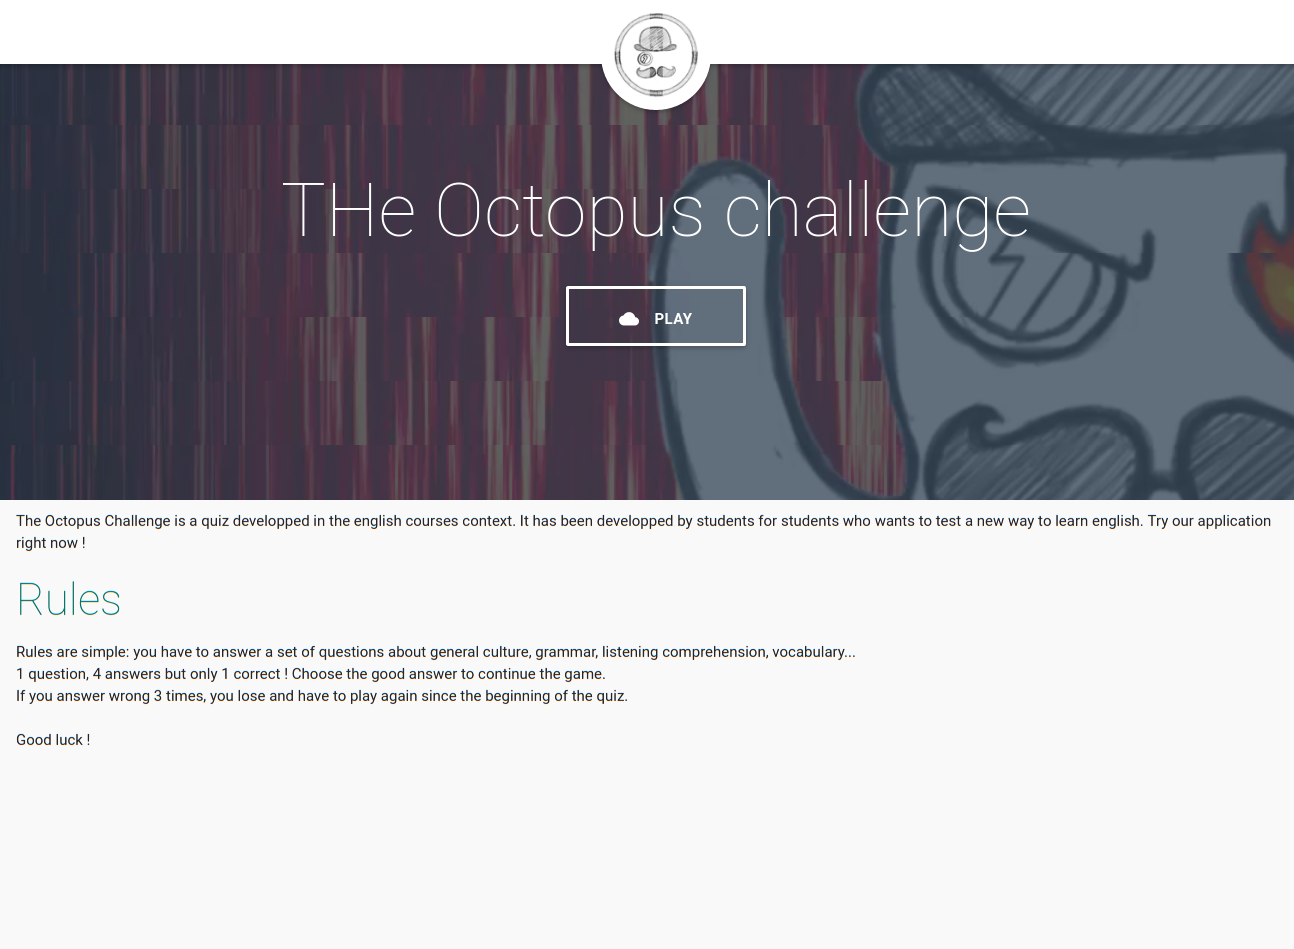
\includegraphics[width=0.8\textwidth]{CHome.png}
		\caption{Home page of the application}
	\end{figure}

The home screen has various sections.
\begin{itemize}
	\item The 'splash screen' section. This animation was designed by us. It aimed at attract players on the website with a surprising video.
	\item The 'Start game' section. This section allows the user to start quiz session.
	%\item The 'Information' section. This section presents rules of the game and the story of \octopusName.
\end{itemize}


	\section{How to play}

To play to \appName, you have to access to the game page via the button 'plays now!'' in the navigation menu or via the play button on the home page.
You can provide a username if you want to share your results at the end of the game.
When you are ready, just click on 'I am ready!' button to start the game session.

\begin{figure} [htbp]
	\centering
	
\includegraphics[width=1\textwidth]{CCreate.png}
	\caption{Form for setting up the game}
\end{figure}

\noindent When you click on 'I am ready!' button, the game starts and a loading screen appears to launch the game.
When the game is launched, the screen is subdivided two screen: the board game containing the current question and the panel containing information of the game session.


\begin{figure} [htbp]
	\centering
	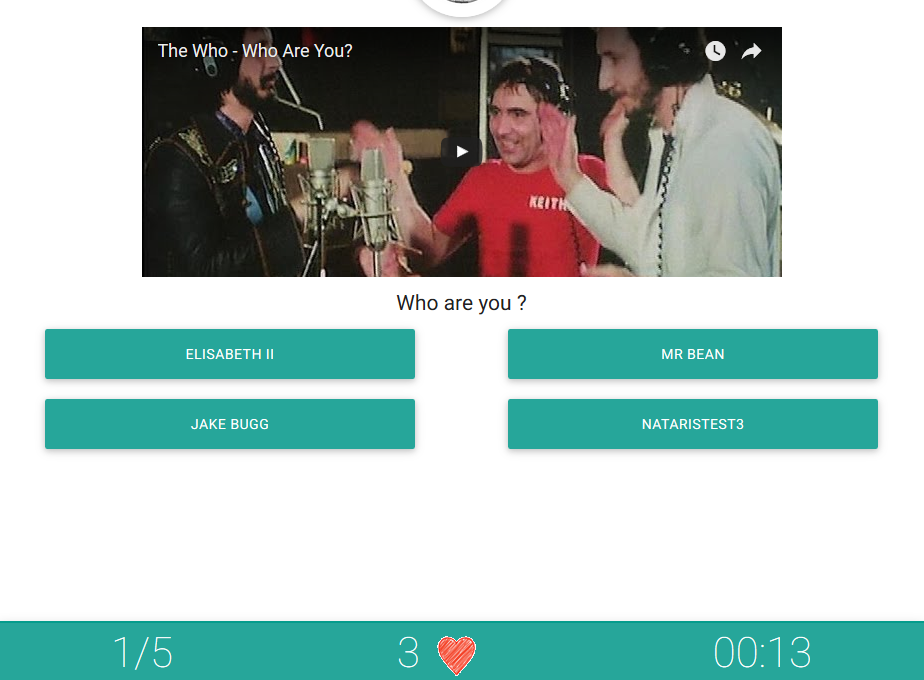
\includegraphics[width=0.8\textwidth]{CGame.png}
	\caption{Game board of the application}
\end{figure}


\subsection{Board game}
The board game shows the current question. In our application, a question is composed of:
\begin{itemize}
	\item An illustration or an extract of a youtube video to have a visual or audio support
	\item The question
	\item Four possibilities of answers
\end{itemize}

\subsection{Information panel}
	During the game, you can see in this panel various information about the game party:
	\begin{itemize}
	\item How many questions you have answered and how many it remain.
	\item How many lives you currently have. At the beginning of the game you have three lives. No life will be given during the game.
	\item A timer to see how many time have past.
	\end{itemize}

To play, just select the correct answer.
If you are right, you go to the next question.
If you are wrong, you lose one of your three lives and an animation appears indicating you chose the wrong answer. You have to choose another proposition until you find the correct answer.
The game continues until you answer all questions or your life drop to zero.
When you finish the quizz, the end screen appears.

\subsection{End of the game}
When you finish the game, you are redirected to the end screen.
\begin{figure} [htbp]
	\centering
	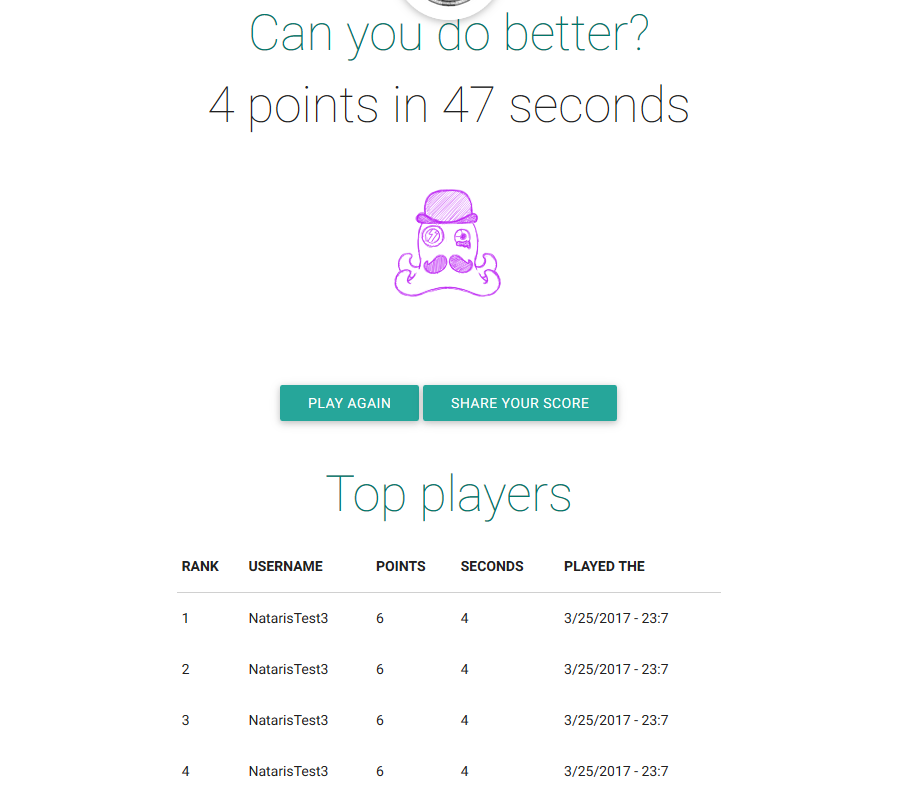
\includegraphics[width=0.7\textwidth]{CEnd.png}
	\caption{Screen of results following the end of the game}
\end{figure}

this screen has:
\begin{itemize}
\item Your score and your time
\item The top player scores
\item Button to replay a party
\item Button to share your score and be in the top 10 players if you have a good score
\end{itemize}

\section{Best scores}
You have the possibility to see top players scores of the application by visiting the appropriate page accessible via the 'high scores' button
When you go to the best score page you can see the best score, and who make it, how many points he got and how many time he makes to answer all questions.
Each column of the array can be sorted by clicking on the column header.

\section{Suggest a question}
If you want to add a question into the game, you can send a question request.
To do this, go to the question request page with the 'suggest a question' button in the navigation bar on the right hand corner.

\begin{figure} [htbp]
	\centering
	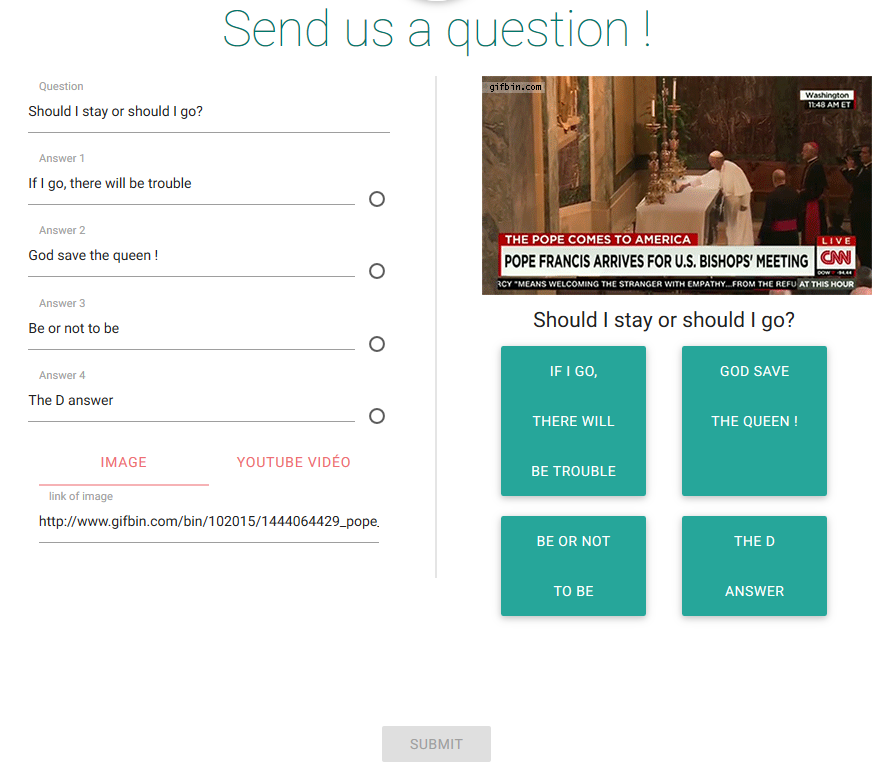
\includegraphics[width=0.9\textwidth]{CQuestion.png}\\
	\caption{Form to fill in for a question request}
\end{figure}

On this page you have a form to indicate all information about the question, the visual,possibilites of answer and a real-time render of the question in the application.
Don't forget to select the correct answer via the checkbox on the right of the answer. When you are satisfied of your question, just click on the submit button to send your question.

\newpage
\chapter{Description technique}

	Ce chapitre présentera en détails les contraintes de ce projet, la manière dont il a été développé ainsi que les problèmes que nous avons dû faire face
	durant les semaines de développement.

	\section{Contraintes}

	Nous avons dégagé deux types de contraintes lors de la phase d'analyse de ce projet:
	\begin{itemize}
		\item Les contraintes liés au sujet (temps de développement, attentes du client).
		\item Les contraintes liés au type de l'outil informatique à développer.\\
	\end{itemize}
Nous avons mis beaucoup de temps à choisir l'outil informatique que nous souhaitions développer. Notre premier choix s'est porté sur un clone du projet Voltair adapté à la langue de Shakespeare.
Cependant, ce choix ne s'est pas révélé motivant. Le choix suivant s'est alors porté sur un quiz à base d'image où l'objectif devait être de trouver le mot corespondant au mot affiché. De plus, ce choix
ne nous semblait pas assez solide pour en faire un outil informatique à part entière. De plus, ce moyen d'apprendre la langue n'est pas forcément efficace.
Notre choix final s'est porté sur un mélange de tous les choix précédents en y apportant quelque chose d'éducatif et simple à utiliser.\\

Le choix du sujet nous a fait perdre du temps pour la conception et le développement de l'outil. Le développement devait donc se faire sur une plus courte période.
Le développement d'une application web s'est alors présenté à nous. Nous disposons tout les deux des compétences pour travailler dans le web.
De plus, le web est accessible depuis n'importe quel appareil disposant d'un navigateur internet, point non négligeable pour le succès de l'application.\\

Le sujet étant fixé, d'autres contraintes se sont rajoutées. La première est le fait que l'application de doit être accessible depuis n'importe quel appareil. En effet,
une application ne fonctionne pas et ne s'affiche pas de la même manière sur un ordinateur ou sur un smartphone (écran plus petit, limitations matérielles...). Il sera donc nécessaire
d'adapter certains aspects de l'application pour la rendre fonctionnelle. La dernière contraintes est l'expérience de l'utilisateur. Si notre application a pour ambition d'améliorer
la compréhension de l'Anglais, la manière dont les informations sont transmises de l'application à l'utilisateur est un point crucial. L'information doit être facilement accessible (peu de clics, accès rapide, application réactive).
Il saura donc important d'adapter l'application afin dé répondre à cette contrainte dans l'objectif d'apporter la meilleure expérience pour l'utilisateur.

\section{Développement de l'application}

L'application \appName \ est composée deux parties:
\begin{itemize}
	\item le back-end, programme étant exécuté sur le serveur, ayant pour but de répondre aux requêtes des clients.
	\item le front-end, programme étant exécuté sur le navigateur web, cœur du projet, permettant de gérer l'affichage des informations sur le navigateur.\\
\end{itemize}


\noindent Pour ce projet, nous avons décidé de développer le back-end avec express, un framework NodeJS permettant de développer rapidement un serveur web. Le serveur permet
\begin{itemize}
	\item D'envoyer le point d'entrée de l'application web avec les programmes du front-end.
	\item De stocker l'ensemble des questions grâce à une base de données.
	\item De stocker l'ensemble des scores des joueurs grâce à une base de données.
	\item d'envoyer l'ensemble des questions disponibles via une API JSON.\\
\end{itemize}

\noindent Pour la base de données, nous avons opté pour PostgreSQL. Ce choix n'a pas d'importance réelle pour l'application mais s'est révélé efficace pour l'hébergement de l'application.
Le serveur est la petite partie de ce projet (environ 300 lignes de code). Le coeur du projet concerne le front-end de l'application (3000 lignes de code).\\

Le front-end a été développé avec VueJS 2. La manière de concevoir des applications web a beaucoup évolué au cours de ces dernières années avec notamment de nombreux frameworks comme AngularS, ReactJS ou encore EmbedJS. VueJS fait partie
de ces frameworks rendant les applications plus maintenables et facile à développer. Le front-end permet:
\begin{itemize}
		\item D'afficher la page correspondante à la requête de l'utilisateur (page d'accueil, jouer, pages des scores ...)
		\item De mettre en oeuvre le moteur de jeu développé pourle quiz (affichage de la question, affichage des réponses, lecture d'une vidéo youtube...)
		\item D'envoyer les résultats d'une partie au serveur
		\item D'afficher le formulaire pour la suggestion d'une question
\end{itemize}


\section{Difficultés rencontrées}

Nous avons dues faire face à deux difficultés au cours de ce projet. La première a été la technologie utilisée pour le développment du front-end. Nous n'avions jamais utilisé ce framework.
Nous avons donc appris comment utiliser VueJS à l'aide de tutoriaux ainsi que des vidéos. Cette difficulté a été cependant fructueuse car elle nous permis d'agrandir notre bagage de compétences
mais également à apprendre une technologie en une courte période.
Le dernier problème dont nous avons dû faire face à la fin du développement de l'application est l'hébergement de cette dernière. Cette étape finale du développement a pour but de
rendre disponible l'application sur internet. De nombreux hébergeurs proposent ce service gratuitement ou non. Cependant, la plupart ne se sont pas tous mis à niveau concernant
les nouvelles technologies comme NodeJS. C'est pourquoi, il a donc été difficile de trouver un hébergeur supportant la technologie comme nous avons employées. Suite à quelques recherches, notre choix s'est cependant tourné vers Heroku,
gratuit et efficace.\\



\section{Identité graphique}
Pour \appName, nous avons voulu adopter un style graphique qui permettrait aux différents éléments de se détacher de l’aspect flat design général utilisé sur l’application.
L’idée retenue parmi tous les styles testés fut des dessins à l’aspect graphique crayonné ou « Draft ».
Nous avons gardé ce style graphique pour plusieurs raisons.
\begin{itemize}
	\item la mascotte du site avait un rendu très intéressant avec ce type de dessin.
	\item Ensuite, le rendu permettait de fournir une image qui se détachait vraiment de l’aspect flat design.
	\item Une facilité de production via une tablette tactile des différents dessins.
	\item pouvoir générer des animations sans pour autant beaucoup travailler la qualité des dessins.
\end{itemize}

%\subsection*{la mascotte}
%Pour l’application \appName, nous voulions intégrer une mascotte au travers laquelle le joueur pourrait s’identifier voir se confronter.\
%Pour cela, nous avions dès le début plusieurs idées de conception, t-elle qu’essayer de la stéréotyper de manière a se qu’elle est un air très british, mais aussi qu’une aptitude sympathique en ressorte.
%Nous sommes donc passées par plusieurs types de mascottes telles qu’un aspect humanoïde, des formes géométriques et enfin la pieuvre.
%Une fois la conception de base réalisée, nous avons eu l’idée de vouloir lui fournir des expressions en fonction des actions du joueur.
%Ainsi nous avons imaginé plusieurs expressions pour \octopusName, qui transite par l’expression faciale, mais aussi par les couleurs utilisées pour le crayonner, de manière à appuyer les sentiments à transmettre. C’est à ce moment que nous avons eu une nouvelle idée pour apporter de la profondeur au sentiment que l’on voulait transmettre, on a alors décidé d’animer les dessins pour former de petit GIF.
%
%\subsection*{Le Logo}
%Pour le logo du site, nous avons dans un premier temps réalisé un logo, dans lequel les éléments distinctifs de la mascotte étaient mis en avant.
%Ensuite, nous avons eu l’idée de promouvoir les pays anglophones au travers de celui-ci en fesse ressortir les différents drapeaux .


\chapter{Conclusion}
\appName \ was a very interesting experience for various reasons.
First of all, it always rewarding to design and developping a software. We had to learn how to use some frameworks, think about how to attract users on the application...
We are very satisfied of the program we made. This first prototype is functional can be used for those who have internet access. Secondly, we have learned from our mistakes we did during the development.
Indeed, we lost a lot of time finding a useful application for us. So, we had to take decisions together to build quickly the application. Finally, the project has been structured in order
to add more features and provide some improvements in a future:
\begin{itemize}
	\item Account system for each user to custom quiz.
	\item Multiplayer quiz session for more fun during the game.
	\item Better user experience on smartphone and tablets.
	\item Voting system in order to add into the game relevant questions of the community.
\end{itemize}

\chapter{annexe}

We used a lot of resources to develop this project.
The following list represents all sources we used to build this application:
\begin{itemize}
	\item 200\% TOEIC 2017 Listening and Reading , Michael Byrne, Michelle Dickinson, Achille Pinson, 2016. used mainly for grammar questions.
	\item \href{http://www.azlyrics.com}{http://www.azlyrics.com}, azlyrics, useful for lyrics of music.
	\item \href{https://vuejs.org/v2/api/}{https://vuejs.org/v2/api/}, API of VueJS, documentation that we have to read to made this project.
	\item \href{http://materializecss.com/}{http://materializecss.com/}, MaterializeCSS, framework based on Material Design to build modern front-end application.
	\item \href{https://www.youtube.com/}{https://www.youtube.com/}, Youtube, used to bring video with a question.
\end{itemize}

\end{document}
